% Options for packages loaded elsewhere
\PassOptionsToPackage{unicode}{hyperref}
\PassOptionsToPackage{hyphens}{url}
%
\documentclass[
]{book}
\title{A Minimal Book Example}
\author{John Doe}
\date{2022-06-08}

\usepackage{amsmath,amssymb}
\usepackage{lmodern}
\usepackage{iftex}
\ifPDFTeX
  \usepackage[T1]{fontenc}
  \usepackage[utf8]{inputenc}
  \usepackage{textcomp} % provide euro and other symbols
\else % if luatex or xetex
  \usepackage{unicode-math}
  \defaultfontfeatures{Scale=MatchLowercase}
  \defaultfontfeatures[\rmfamily]{Ligatures=TeX,Scale=1}
\fi
% Use upquote if available, for straight quotes in verbatim environments
\IfFileExists{upquote.sty}{\usepackage{upquote}}{}
\IfFileExists{microtype.sty}{% use microtype if available
  \usepackage[]{microtype}
  \UseMicrotypeSet[protrusion]{basicmath} % disable protrusion for tt fonts
}{}
\makeatletter
\@ifundefined{KOMAClassName}{% if non-KOMA class
  \IfFileExists{parskip.sty}{%
    \usepackage{parskip}
  }{% else
    \setlength{\parindent}{0pt}
    \setlength{\parskip}{6pt plus 2pt minus 1pt}}
}{% if KOMA class
  \KOMAoptions{parskip=half}}
\makeatother
\usepackage{xcolor}
\IfFileExists{xurl.sty}{\usepackage{xurl}}{} % add URL line breaks if available
\IfFileExists{bookmark.sty}{\usepackage{bookmark}}{\usepackage{hyperref}}
\hypersetup{
  pdftitle={A Minimal Book Example},
  pdfauthor={John Doe},
  hidelinks,
  pdfcreator={LaTeX via pandoc}}
\urlstyle{same} % disable monospaced font for URLs
\usepackage{color}
\usepackage{fancyvrb}
\newcommand{\VerbBar}{|}
\newcommand{\VERB}{\Verb[commandchars=\\\{\}]}
\DefineVerbatimEnvironment{Highlighting}{Verbatim}{commandchars=\\\{\}}
% Add ',fontsize=\small' for more characters per line
\usepackage{framed}
\definecolor{shadecolor}{RGB}{248,248,248}
\newenvironment{Shaded}{\begin{snugshade}}{\end{snugshade}}
\newcommand{\AlertTok}[1]{\textcolor[rgb]{0.94,0.16,0.16}{#1}}
\newcommand{\AnnotationTok}[1]{\textcolor[rgb]{0.56,0.35,0.01}{\textbf{\textit{#1}}}}
\newcommand{\AttributeTok}[1]{\textcolor[rgb]{0.77,0.63,0.00}{#1}}
\newcommand{\BaseNTok}[1]{\textcolor[rgb]{0.00,0.00,0.81}{#1}}
\newcommand{\BuiltInTok}[1]{#1}
\newcommand{\CharTok}[1]{\textcolor[rgb]{0.31,0.60,0.02}{#1}}
\newcommand{\CommentTok}[1]{\textcolor[rgb]{0.56,0.35,0.01}{\textit{#1}}}
\newcommand{\CommentVarTok}[1]{\textcolor[rgb]{0.56,0.35,0.01}{\textbf{\textit{#1}}}}
\newcommand{\ConstantTok}[1]{\textcolor[rgb]{0.00,0.00,0.00}{#1}}
\newcommand{\ControlFlowTok}[1]{\textcolor[rgb]{0.13,0.29,0.53}{\textbf{#1}}}
\newcommand{\DataTypeTok}[1]{\textcolor[rgb]{0.13,0.29,0.53}{#1}}
\newcommand{\DecValTok}[1]{\textcolor[rgb]{0.00,0.00,0.81}{#1}}
\newcommand{\DocumentationTok}[1]{\textcolor[rgb]{0.56,0.35,0.01}{\textbf{\textit{#1}}}}
\newcommand{\ErrorTok}[1]{\textcolor[rgb]{0.64,0.00,0.00}{\textbf{#1}}}
\newcommand{\ExtensionTok}[1]{#1}
\newcommand{\FloatTok}[1]{\textcolor[rgb]{0.00,0.00,0.81}{#1}}
\newcommand{\FunctionTok}[1]{\textcolor[rgb]{0.00,0.00,0.00}{#1}}
\newcommand{\ImportTok}[1]{#1}
\newcommand{\InformationTok}[1]{\textcolor[rgb]{0.56,0.35,0.01}{\textbf{\textit{#1}}}}
\newcommand{\KeywordTok}[1]{\textcolor[rgb]{0.13,0.29,0.53}{\textbf{#1}}}
\newcommand{\NormalTok}[1]{#1}
\newcommand{\OperatorTok}[1]{\textcolor[rgb]{0.81,0.36,0.00}{\textbf{#1}}}
\newcommand{\OtherTok}[1]{\textcolor[rgb]{0.56,0.35,0.01}{#1}}
\newcommand{\PreprocessorTok}[1]{\textcolor[rgb]{0.56,0.35,0.01}{\textit{#1}}}
\newcommand{\RegionMarkerTok}[1]{#1}
\newcommand{\SpecialCharTok}[1]{\textcolor[rgb]{0.00,0.00,0.00}{#1}}
\newcommand{\SpecialStringTok}[1]{\textcolor[rgb]{0.31,0.60,0.02}{#1}}
\newcommand{\StringTok}[1]{\textcolor[rgb]{0.31,0.60,0.02}{#1}}
\newcommand{\VariableTok}[1]{\textcolor[rgb]{0.00,0.00,0.00}{#1}}
\newcommand{\VerbatimStringTok}[1]{\textcolor[rgb]{0.31,0.60,0.02}{#1}}
\newcommand{\WarningTok}[1]{\textcolor[rgb]{0.56,0.35,0.01}{\textbf{\textit{#1}}}}
\usepackage{longtable,booktabs,array}
\usepackage{calc} % for calculating minipage widths
% Correct order of tables after \paragraph or \subparagraph
\usepackage{etoolbox}
\makeatletter
\patchcmd\longtable{\par}{\if@noskipsec\mbox{}\fi\par}{}{}
\makeatother
% Allow footnotes in longtable head/foot
\IfFileExists{footnotehyper.sty}{\usepackage{footnotehyper}}{\usepackage{footnote}}
\makesavenoteenv{longtable}
\usepackage{graphicx}
\makeatletter
\def\maxwidth{\ifdim\Gin@nat@width>\linewidth\linewidth\else\Gin@nat@width\fi}
\def\maxheight{\ifdim\Gin@nat@height>\textheight\textheight\else\Gin@nat@height\fi}
\makeatother
% Scale images if necessary, so that they will not overflow the page
% margins by default, and it is still possible to overwrite the defaults
% using explicit options in \includegraphics[width, height, ...]{}
\setkeys{Gin}{width=\maxwidth,height=\maxheight,keepaspectratio}
% Set default figure placement to htbp
\makeatletter
\def\fps@figure{htbp}
\makeatother
\setlength{\emergencystretch}{3em} % prevent overfull lines
\providecommand{\tightlist}{%
  \setlength{\itemsep}{0pt}\setlength{\parskip}{0pt}}
\setcounter{secnumdepth}{5}
\usepackage{booktabs}
\usepackage{amsthm}
\usepackage{zi4}
\usepackage[hangul]{kotex}
\usepackage{fontspec}
\makeatletter
\def\thm@space@setup{%
  \thm@preskip=8pt plus 2pt minus 4pt
  \thm@postskip=\thm@preskip
}
\makeatother
\ifLuaTeX
  \usepackage{selnolig}  % disable illegal ligatures
\fi
\usepackage[]{natbib}
\bibliographystyle{plainnat}

\usepackage{amsthm}
\newtheorem{theorem}{Theorem}[chapter]
\newtheorem{lemma}{Lemma}[chapter]
\newtheorem{corollary}{Corollary}[chapter]
\newtheorem{proposition}{Proposition}[chapter]
\newtheorem{conjecture}{Conjecture}[chapter]
\theoremstyle{definition}
\newtheorem{definition}{Definition}[chapter]
\theoremstyle{definition}
\newtheorem{example}{Example}[chapter]
\theoremstyle{definition}
\newtheorem{exercise}{Exercise}[chapter]
\theoremstyle{definition}
\newtheorem{hypothesis}{Hypothesis}[chapter]
\theoremstyle{remark}
\newtheorem*{remark}{Remark}
\newtheorem*{solution}{Solution}
\begin{document}
\maketitle

{
\setcounter{tocdepth}{1}
\tableofcontents
}
\hypertarget{about}{%
\chapter{About}\label{about}}

This is a \emph{sample} book written in \textbf{Markdown}. You can use anything that Pandoc's Markdown supports; for example, a math equation \(a^2 + b^2 = c^2\).

\hypertarget{usage}{%
\section{Usage}\label{usage}}

Each \textbf{bookdown} chapter is an .Rmd file, and each .Rmd file can contain one (and only one) chapter. A chapter \emph{must} start with a first-level heading: \texttt{\#\ A\ good\ chapter}, and can contain one (and only one) first-level heading.

Use second-level and higher headings within chapters like: \texttt{\#\#\ A\ short\ section} or \texttt{\#\#\#\ An\ even\ shorter\ section}.

The \texttt{index.Rmd} file is required, and is also your first book chapter. It will be the homepage when you render the book.

\hypertarget{render-book}{%
\section{Render book}\label{render-book}}

You can render the HTML version of this example book without changing anything:

\begin{enumerate}
\def\labelenumi{\arabic{enumi}.}
\item
  Find the \textbf{Build} pane in the RStudio IDE, and
\item
  Click on \textbf{Build Book}, then select your output format, or select ``All formats'' if you'd like to use multiple formats from the same book source files.
\end{enumerate}

Or build the book from the R console:

\begin{Shaded}
\begin{Highlighting}[]
\NormalTok{bookdown}\SpecialCharTok{::}\FunctionTok{render\_book}\NormalTok{()}
\end{Highlighting}
\end{Shaded}

To render this example to PDF as a \texttt{bookdown::pdf\_book}, you'll need to install XeLaTeX. You are recommended to install TinyTeX (which includes XeLaTeX): \url{https://yihui.org/tinytex/}.

\hypertarget{preview-book}{%
\section{Preview book}\label{preview-book}}

As you work, you may start a local server to live preview this HTML book. This preview will update as you edit the book when you save individual .Rmd files. You can start the server in a work session by using the RStudio add-in ``Preview book'', or from the R console:

\begin{Shaded}
\begin{Highlighting}[]
\NormalTok{bookdown}\SpecialCharTok{::}\FunctionTok{serve\_book}\NormalTok{()}
\end{Highlighting}
\end{Shaded}

\mainmatter

\hypertarget{intro}{%
\chapter{Introduction}\label{intro}}

이 책을 쓰게 된 계기는 간단하다. 약 6년간 서울대학교 산업인력개발 전공의 학부와 대학원 통계 수업을 진행하면서 인력개발 분야의 통계 서적의 필요성을 실감했기 떄문이다. 기존의 서적들을 각기 조합하여 수업을 진행하다보니, 학생들은 물론 교수자도 힘들었던 점들이 많았다. 수많은 서적들이 제각기의 시각으로 통계 관련 이론과 실무적인 내용들을 잘 풀어내고 있지만, 우리 분야에 적합한 책을 찾기는 어려웠다. 두번째 이유는 코로나로 인해 대부분의 출장과 회의가 온라인으로 이뤄지면서, 이동시간이 절약되어 집필에 필요한 시간이 확보되었다.

이 책은 일종의 조각 모음으로 집필이 진행되었다. 매년 수업을 진행하며 조각 조각 만들어냈던 자료들을 통합함으로서 하나의 스토리를 만들어내고자 노력했다. 개인적으로는 통계 전공자가 아니기 때문에 이 책을 쓰는데 부담이 없지 않았다. 따라서 오류를 최소화하기 위해 집필의 말미에는 각 분야별 전문가 분들께 크로스체크를 부탁하였다.

\hypertarget{ruxc744-uxc65c-uxc0acuxc6a9uxd574uxc57cuxd560uxae4c}{%
\section{R을 왜 사용해야할까?}\label{ruxc744-uxc65c-uxc0acuxc6a9uxd574uxc57cuxd560uxae4c}}

책의 제목에서 알 수 있듯이 기본이 되는 통계 패키지는 R을 사용하였다. 사실 교육학 분야의 많은 오래된 학자들은 SPSS가 익숙하고, 나 역시 첫 통계 공부는 SPSS로 시작했다. 관행은 계기가 없으면 바뀌기 어렵기 때문에, 학교에 부임한 이후에도 수년간은 SPSS를 이용한 수업을 진행하기도 했다. 하지만 다음과 같은 네 가지 이유로 SPSS는 나의 컴퓨터에서 사라지게 되었다.

\begin{itemize}
\item
  첫째, SPSSS는 비싼 라이센스를 사용해야 하기 떄문에 개인 연구자에 적합하지 않다. 서울대 역시 SPSS 제조사와 지리한 라이선스 가격 협상을 이어가고 있는 실정이다. 하물며 개인이 라이센스에 지갑을 열어야 하는 경우 SPSS는 좋은 선택이 아니다.
\item
  둘째, SPSS가 갖고 있는 직관적인 인터페이스와 간단한 분석방법은 종종 초보 연구자의 오류를 촉진한다. 모든 종류의 프로그램이 그렇듯이 이들은 분석의 적합성을 검토해주지 않는다. 자판기에 동전을 넣으면 음료수가 나오듯이 데이터를 입력하면 분석결과가 나오지만, 그것이 잘못된 선택인지 알수가 없다. 반면에 R 등의 스크립트 기반의 통계패키지는 적어도 내가 무엇을 분석하려고 하는지에 대한 기본적인 이해를 필요로 한다.
\item
  셋째, 복잡한 분석(이라 쓰고 삽질이라 읽는다)을 실시할 때 click to click 방식의 통계패키지는 삽질의 시간을 더 길게 만든다. 보통 우리가 마주하는 데이터는 다양한 변형(manipulation)을 요구하는데, 이때 (1) 어떠한 형태로 데이터를 변형할 것인지, (2) 변형을 위한 각 단계는 어떻게 구성해야 하는지에 대한 사전정보를 알고 있는 경우는 드물다. R과 같이 스크립트를 기반으로 데이터를 핸들링하고 분석할 수 있는 경우는 일주일간 작업한 내용의 오류를 발견했을 때, 그간 작성해놓은 코드에 일부만 수정하고 실행함으로서 간단히 오류를 고칠 수 있다. SPSS 같은 프로그램들은 데이터 변형 및 분석의 복원이 불가능하다는 점을 고려해보면 어마어마한 장점이 아닐 수 있다. 보통 이런 작업을 디버깅(debuging)이라고 하는데, 고통스러운 디버깅 작업을 10시간정도 하게 되면, R을 시작하는데 필요한 약간의 허들은 쉽게 느껴질 것이다.
\item
  넷째, R은 빠르게 변화하는 최신 분석기법들을 빠르게 설치, 활용할 수 있다. 종종 R을 스마트폰에 비유하곤하는데, ios나 android와 같은 플랫폼에 여러가지 어플을 설치하는 방식을 생각하면 간단하다. 플랫폼의 업데이트는 느리고 무겁지만, 각각의 어플은 가볍고, 빠르며, 쉽게 적용이 가능하다. 결국 확장성의 장점이 R이 갖고 있는 가장 큰 장점이라고 볼 수 있다.
\end{itemize}

R의 기본적인 설치, 구조 이해, 분석의 기초와 함께, 이 책에서는 통계학의 기본적인 내용들도 알기 쉽게 설명하고자 노력했다. 두 내용 모두 방대하기 때문에 보통 하나의 책에서 통계패키지의 분석 테크닉과 통계학 이론을 한꺼 번에 다루지는 않는다. 하지만 수년간 학생들을 가르치다보니 두 내용을 연결하는 책이 절실하게 필요했다. 두마리의 토끼를 과연 잡았을지는 모르겠지만, 부디 이 책이 의도한 바를 달성했기를 바란다.

\hypertarget{uxc774-uxcc45uxc758-uxad6cuxc131}{%
\section{이 책의 구성}\label{uxc774-uxcc45uxc758-uxad6cuxc131}}

이 책은 크게 3부로 구성된다.

\hypertarget{uxbd80.-ruxc758-uxae30uxcd08-uxc774uxd574}{%
\subsection*{1부. R의 기초 이해}\label{uxbd80.-ruxc758-uxae30uxcd08-uxc774uxd574}}
\addcontentsline{toc}{subsection}{1부. R의 기초 이해}

1부는 R이라는 데이터 분석 도구tool에 대해 이해하도록 한다. 앞서 언급했던것처럼 R은 특히 복잡한 데이터 전처리에서 진가를 발휘한다. 우리가 접하는 데이터들은 전처리가 거의 필요없는 유형(내 연구 가설에 딱 맞는 형태로 직접 수집한 데이터, 예를 들어 학위논문 등을 위해 직접 수집해서 코딩까지한 자료)부터 매우 복잡한 전처리를 해야만 분석이 가능한 유형(보통 행정 및 관리를 위해 조직에 축적된 chunky한 데이터들)까지 다양하다. 1부에서는 이러한 데이터 전처리를 용이하게 하기 위해 필요한 다양한 기법들에 대해 소개할 예정이다. 1부에서 다룰 내용들은 다음과 같다.

\begin{itemize}
\tightlist
\item
  1장. R설치, 작업환경 셋업과 R 환경이해하기
\item
  2장. R 자료 구조의 이해
\item
  3장. R을 활용한 데이터 전처리
\item
  4장. R을 활용한 데이터 시각화
\end{itemize}

\hypertarget{uxbd80.-ruxc744-uxd65cuxc6a9uxd55c-uxae30uxcd08-uxb2e4uxbcc0uxb7c9-uxbd84uxc11d}{%
\subsection*{2부. R을 활용한 기초 다변량 분석}\label{uxbd80.-ruxc744-uxd65cuxc6a9uxd55c-uxae30uxcd08-uxb2e4uxbcc0uxb7c9-uxbd84uxc11d}}
\addcontentsline{toc}{subsection}{2부. R을 활용한 기초 다변량 분석}

2부는 연구를 위해 활용되는 다양한 다변량 분석 기법의 이론에 대해 소개한다. 1부는 R이라는 분석도구를 사용하는 테크닉에 대한 소개일 뿐이다. 다시 말해 못을 박는 망치 사용법일뿐이지 어디에다 못을 박아야 하는지, 몇개를 박아야 하는지, 얼마나 깊숙히 박아야 하는지에 대한 답을 주지는 못한다. 2부에서는 추론통계와 가설 검정에 대한 이해를 바탕으로 t검정과 ANOVA, 상관분석, 회귀분석, 로지스틱, 매개분석과 조절분석에 대해 다룰 예정이다. 이 밖에 더 많은 다변량 분석기법들이 존재하지만, 산업인력개발 분야에서 가장 빈번하게 다루는 기초적인 분석기법들을 선택하였다. 각 장별로 개념이해, 결과 해석, R을 활용한 분석코드 순서로 기술되었다.

\begin{itemize}
\tightlist
\item
  5장. 추론통계와 가설검정
\item
  6장. t 검정과 ANOVA
\item
  7장. 상관분석
\item
  8장. 회귀분석
\item
  9장. 로지스틱 회귀분석
\item
  10장. 매개분석과 조절분석
\item
  11장. 구조방정식 (????)
\end{itemize}

\hypertarget{uxbd80.-uxc2e4uxc804uxb370uxc774uxd130uxb97c-uxd65cuxc6a9uxd55c-uxbd84uxc11d-uxc0acuxb840}{%
\subsection*{3부. 실전데이터를 활용한 분석 사례}\label{uxbd80.-uxc2e4uxc804uxb370uxc774uxd130uxb97c-uxd65cuxc6a9uxd55c-uxbd84uxc11d-uxc0acuxb840}}
\addcontentsline{toc}{subsection}{3부. 실전데이터를 활용한 분석 사례}

\hypertarget{uxbc30uxc6b0uxc9c0-uxc54auxb294-uxb0b4uxc6a9uxb4e4}{%
\section{배우지 않는 내용들}\label{uxbc30uxc6b0uxc9c0-uxc54auxb294-uxb0b4uxc6a9uxb4e4}}

\begin{verbatim}
what did you say ?    
\end{verbatim}

이 책에서 다루지 않는 내용은 그야말로 산더미 같이 많이 있다. 정확히 숫자로 표현 할수는 없겠지만 한 90\%정도는 책에 담지 못한 내용들일 것이다!! 아마 10년정도 후에는 99\% 정도로 늘어날지 모르겠다. 하지만 이 책에 담긴 내용들을 충분히 숙지하였다면 나머지 90\%의 내용은 여러분 스스로 학습할 수 있는 좋은 기본기를 갖췄다고 생각해도 무방하다. 개인적으로는 이 책이 (1) 여러분들의 통계포비아를 없애주고, (2) 새로운 개념, 기법에 대한 자기주도학습이 가능하도록 하는 일종의 밑바탕으로 기능했으면 하는 바램이다.

좀 더 구체적으로 이 책에서 제외된 내용은 다음과 같다. 우선 1부에서 R을 활용한 데이터 전처리의 맛보기만 기술하였기 때문에, 이른바 빅데이터라고 불리는 청키한 데이터를 다루는 기법까지 설명하지는 못했다. 특히 다양한 DB 등에서 데이터를 끌어와 분석에 용이한 형태로 만드는 것은 좀더 심화된 기법이 필요하다. 이와 관련해서는 관련한 기존 서적들을 충분히 참조했으면 하는 바람이다(물론 1부를 모두 이해한 후에)

2부에서도 다루지 못한 내용들이 많다. 특히 15년 전부터 사회과학분야에 거대한 유행으로 자리잡은 구조방정식structural equaation modeling, 다층선형모형hierarchical linear modeling 등 굵직한 기법들이 모두 빠져있다. 이러한 분석기법들은 각각의 대표적인 기본서들이 있으므로, 이를 참조하였으면 하는 바람이다. 이들 역시 일종의 회귀분석의 변형이기 때문에 기초를 탄탄하게 쌓았다면 이해를 확장하는데 어려움이 없을 것이라 생각한다. 이와 더불어 다양한 longitudinal data를 다루는 분석기법들도 생략되어 있다.

이밖에도 저자의 또 다른 강의인 ``직업연구''나 ``산업인력개발 노동시장분석론''에서 다루었던 다양한 통계기법에 대한 내용들도 빠져있다. 아마도 빠른 시간 안에 위의 두 강의에서 다루었던 내용을 별도의 책으로 출간할 수 있지 않을 까 기대한다(기대만 하고 있다\ldots.)

\hypertarget{uxb2f9uxbd80uxc758-uxb9d0}{%
\section{당부의 말}\label{uxb2f9uxbd80uxc758-uxb9d0}}

마지막으로 우연히 이 책을 접한 독자들에게 하고 싶은 말은 책의 내용을 이해하는 것을 포기 하지 말라는 것이다. 고등학교 때 '수학의 정석'의 첫 챕터인 집합 부분만 까맣게 손때가 묻어있던것을 기억할 것이다. 많은 사람들이 2부의 첫 챕터에서 흥미를 잃겠지만, 포기하지 않고 여러번 완독을 한다면 분명 많은 도움이 될 것이다. 설사 이해하지 못하는 내용이 있다하더라도 여러번 읽고, 손으로 문제를 풀어보는 버릇을 들이면 더 빠르게 이해할 수 있다.

또 간단한 소논문 등을 작성해보고 다시 책을 읽어보면 이해가 안되었던 부분들이 새롭게 보이는 날들이 있을 것이라 믿어 의심치 않는다. 또한 이 책이 정답이 아니므로, 설명이 부족한 부분들이 있다면 구글이나 유튜브 등에 키워드 검색을 통해 추가적인 설명자료와 강의등의 도움을 받길 바란다.

\hypertarget{cross}{%
\chapter{Cross-references}\label{cross}}

Cross-references make it easier for your readers to find and link to elements in your book.

\hypertarget{chapters-and-sub-chapters}{%
\section{Chapters and sub-chapters}\label{chapters-and-sub-chapters}}

There are two steps to cross-reference any heading:

\begin{enumerate}
\def\labelenumi{\arabic{enumi}.}
\tightlist
\item
  Label the heading: \texttt{\#\ Hello\ world\ \{\#nice-label\}}.

  \begin{itemize}
  \tightlist
  \item
    Leave the label off if you like the automated heading generated based on your heading title: for example, \texttt{\#\ Hello\ world} = \texttt{\#\ Hello\ world\ \{\#hello-world\}}.
  \item
    To label an un-numbered heading, use: \texttt{\#\ Hello\ world\ \{-\#nice-label\}} or \texttt{\{\#\ Hello\ world\ .unnumbered\}}.
  \end{itemize}
\item
  Next, reference the labeled heading anywhere in the text using \texttt{\textbackslash{}@ref(nice-label)}; for example, please see Chapter \ref{cross}.

  \begin{itemize}
  \tightlist
  \item
    If you prefer text as the link instead of a numbered reference use: \protect\hyperlink{cross}{any text you want can go here}.
  \end{itemize}
\end{enumerate}

\hypertarget{captioned-figures-and-tables}{%
\section{Captioned figures and tables}\label{captioned-figures-and-tables}}

Figures and tables \emph{with captions} can also be cross-referenced from elsewhere in your book using \texttt{\textbackslash{}@ref(fig:chunk-label)} and \texttt{\textbackslash{}@ref(tab:chunk-label)}, respectively.

See Figure \ref{fig:nice-fig}.

\begin{Shaded}
\begin{Highlighting}[]
\FunctionTok{par}\NormalTok{(}\AttributeTok{mar =} \FunctionTok{c}\NormalTok{(}\DecValTok{4}\NormalTok{, }\DecValTok{4}\NormalTok{, .}\DecValTok{1}\NormalTok{, .}\DecValTok{1}\NormalTok{))}
\FunctionTok{plot}\NormalTok{(pressure, }\AttributeTok{type =} \StringTok{\textquotesingle{}b\textquotesingle{}}\NormalTok{, }\AttributeTok{pch =} \DecValTok{19}\NormalTok{)}
\end{Highlighting}
\end{Shaded}

\begin{figure}

{\centering 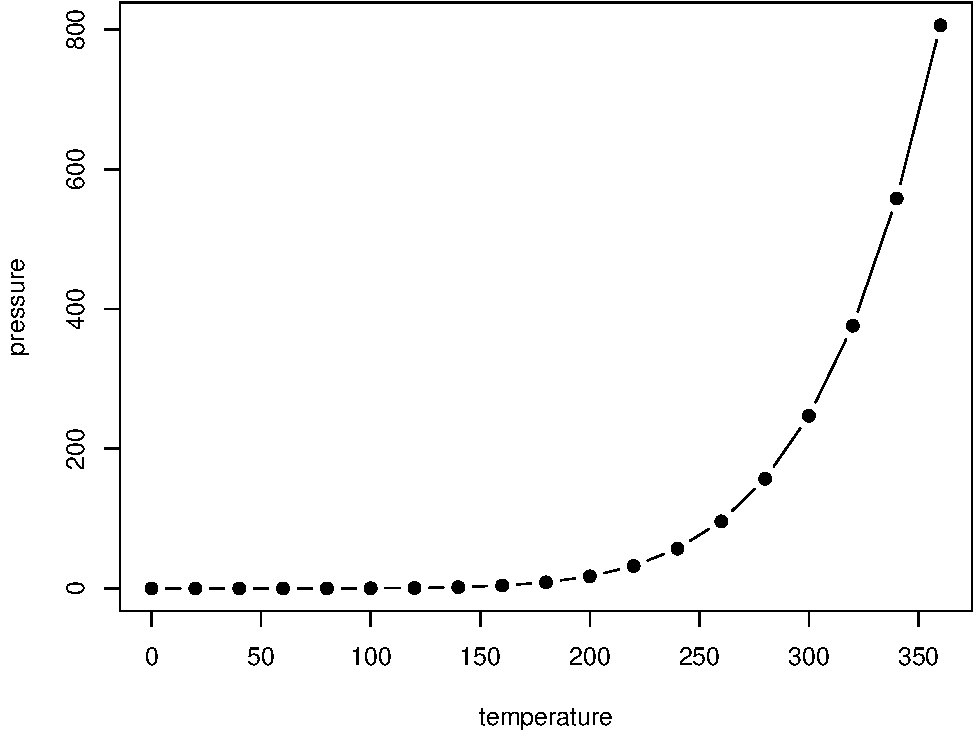
\includegraphics[width=0.8\linewidth]{_main_files/figure-latex/nice-fig-1} 

}

\caption{Here is a nice figure!}\label{fig:nice-fig}
\end{figure}

Don't miss Table \ref{tab:nice-tab}.

\begin{Shaded}
\begin{Highlighting}[]
\NormalTok{knitr}\SpecialCharTok{::}\FunctionTok{kable}\NormalTok{(}
  \FunctionTok{head}\NormalTok{(pressure, }\DecValTok{10}\NormalTok{), }\AttributeTok{caption =} \StringTok{\textquotesingle{}Here is a nice table!\textquotesingle{}}\NormalTok{,}
  \AttributeTok{booktabs =} \ConstantTok{TRUE}
\NormalTok{)}
\end{Highlighting}
\end{Shaded}

\begin{table}

\caption{\label{tab:nice-tab}Here is a nice table!}
\centering
\begin{tabular}[t]{rr}
\toprule
temperature & pressure\\
\midrule
0 & 0.0002\\
20 & 0.0012\\
40 & 0.0060\\
60 & 0.0300\\
80 & 0.0900\\
\addlinespace
100 & 0.2700\\
120 & 0.7500\\
140 & 1.8500\\
160 & 4.2000\\
180 & 8.8000\\
\bottomrule
\end{tabular}
\end{table}

\hypertarget{parts}{%
\chapter{Parts}\label{parts}}

You can add parts to organize one or more book chapters together. Parts can be inserted at the top of an .Rmd file, before the first-level chapter heading in that same file.

Add a numbered part: \texttt{\#\ (PART)\ Act\ one\ \{-\}} (followed by \texttt{\#\ A\ chapter})

Add an unnumbered part: \texttt{\#\ (PART\textbackslash{}*)\ Act\ one\ \{-\}} (followed by \texttt{\#\ A\ chapter})

Add an appendix as a special kind of un-numbered part: \texttt{\#\ (APPENDIX)\ Other\ stuff\ \{-\}} (followed by \texttt{\#\ A\ chapter}). Chapters in an appendix are prepended with letters instead of numbers.

\hypertarget{footnotes-and-citations}{%
\chapter{Footnotes and citations}\label{footnotes-and-citations}}

\hypertarget{footnotes}{%
\section{Footnotes}\label{footnotes}}

Footnotes are put inside the square brackets after a caret \texttt{\^{}{[}{]}}. Like this one \footnote{This is a footnote.}.

\hypertarget{citations}{%
\section{Citations}\label{citations}}

Reference items in your bibliography file(s) using \texttt{@key}.

For example, we are using the \textbf{bookdown} package \citep{R-bookdown} (check out the last code chunk in index.Rmd to see how this citation key was added) in this sample book, which was built on top of R Markdown and \textbf{knitr} \citep{xie2015} (this citation was added manually in an external file book.bib).
Note that the \texttt{.bib} files need to be listed in the index.Rmd with the YAML \texttt{bibliography} key.

The RStudio Visual Markdown Editor can also make it easier to insert citations: \url{https://rstudio.github.io/visual-markdown-editing/\#/citations}

\hypertarget{blocks}{%
\chapter{Blocks}\label{blocks}}

\hypertarget{equations}{%
\section{Equations}\label{equations}}

Here is an equation.

\begin{equation} 
  f\left(k\right) = \binom{n}{k} p^k\left(1-p\right)^{n-k}
  \label{eq:binom}
\end{equation}

You may refer to using \texttt{\textbackslash{}@ref(eq:binom)}, like see Equation \eqref{eq:binom}.

\hypertarget{theorems-and-proofs}{%
\section{Theorems and proofs}\label{theorems-and-proofs}}

Labeled theorems can be referenced in text using \texttt{\textbackslash{}@ref(thm:tri)}, for example, check out this smart theorem \ref{thm:tri}.

\begin{theorem}
\protect\hypertarget{thm:tri}{}\label{thm:tri}For a right triangle, if \(c\) denotes the \emph{length} of the hypotenuse
and \(a\) and \(b\) denote the lengths of the \textbf{other} two sides, we have
\[a^2 + b^2 = c^2\]
\end{theorem}

Read more here \url{https://bookdown.org/yihui/bookdown/markdown-extensions-by-bookdown.html}.

\hypertarget{callout-blocks}{%
\section{Callout blocks}\label{callout-blocks}}

The R Markdown Cookbook provides more help on how to use custom blocks to design your own callouts: \url{https://bookdown.org/yihui/rmarkdown-cookbook/custom-blocks.html}

\hypertarget{sharing-your-book}{%
\chapter{Sharing your book}\label{sharing-your-book}}

\hypertarget{publishing}{%
\section{Publishing}\label{publishing}}

HTML books can be published online, see: \url{https://bookdown.org/yihui/bookdown/publishing.html}

\hypertarget{pages}{%
\section{404 pages}\label{pages}}

By default, users will be directed to a 404 page if they try to access a webpage that cannot be found. If you'd like to customize your 404 page instead of using the default, you may add either a \texttt{\_404.Rmd} or \texttt{\_404.md} file to your project root and use code and/or Markdown syntax.

\hypertarget{metadata-for-sharing}{%
\section{Metadata for sharing}\label{metadata-for-sharing}}

Bookdown HTML books will provide HTML metadata for social sharing on platforms like Twitter, Facebook, and LinkedIn, using information you provide in the \texttt{index.Rmd} YAML. To setup, set the \texttt{url} for your book and the path to your \texttt{cover-image} file. Your book's \texttt{title} and \texttt{description} are also used.

This \texttt{gitbook} uses the same social sharing data across all chapters in your book- all links shared will look the same.

Specify your book's source repository on GitHub using the \texttt{edit} key under the configuration options in the \texttt{\_output.yml} file, which allows users to suggest an edit by linking to a chapter's source file.

Read more about the features of this output format here:

\url{https://pkgs.rstudio.com/bookdown/reference/gitbook.html}

Or use:

\begin{Shaded}
\begin{Highlighting}[]
\NormalTok{?bookdown}\SpecialCharTok{::}\NormalTok{gitbook}
\end{Highlighting}
\end{Shaded}


  \bibliography{book.bib,packages.bib}

\end{document}
